% ---------------------------------------------------------------------------
% intro_and_figures.tex -- introduction + three results figures for the
% scaffold manuscript. Drafted 2026-08-26 on branch sycophancy-scenario-redesign.
%
% DATA PROVENANCE. Every number in Figures 1-2 is generated from committed
% artifacts and was re-verified on the day of drafting:
%   Fig 1: analyze_length_matched_elephant --corrected  (truncation-corrected
%          arm-level validation deltas, ELEPHANT-OEQ, 150 items/arm)
%   Fig 2: divergence_study_outputs/subinstruction_attribution.csv
%          (n=90 per cell, claude-sonnet-4-6)
%   Fig 3: divergence_study_outputs/bm_neutral_{standard,oneline,ncot}.json
%          (matched three-arm forced-verdict run, 2026-08-26; n=600 units
%          per arm, shared items). The run REVERSED the drafted claim: NoT
%          RAISES false-premise affirmation. The one_line arm was generated
%          with the standard prompt via a PROMPTS-key fallback and is
%          reported as a second untreated replicate. The older triage-cache
%          value (0.287, n=171, different item sample and selection config)
%          is disclosed as a discrepancy note and never mixed in. CIs are
%          item-clustered bootstrap, 10k draws (analyze_bm_embodiment.py).
%
% Requires: pgfplots (\pgfplotsset{compat=1.17} or later).
% ---------------------------------------------------------------------------

% ================= MATCHED THREE-ARM RUN (2026-08-26) =======================
\newcommand{\pTrueStd}{0.157}      % bm_neutral_standard.json, n=600
\newcommand{\pTrueStdRep}{0.147}   % bm_neutral_oneline.json: untreated REPLICATE
\newcommand{\pTrueNoT}{0.223}      % bm_neutral_ncot.json, n=600

% =========================== INTRODUCTION ===================================
\section{Introduction}
\label{sec:intro}

When a person brings a language model an account of their own conflict and
asks who was in the wrong, the model's answer is systematically gentler than
the answer it gives a bystander who presents the identical text. This is
sycophancy in its consequential form: not flattery as a style, but deference
that changes what an adviser is willing to conclude, precisely for the person
who most needs the conclusion to be honest. Reinforcement from human feedback
plausibly builds the behaviour in --- approval is the training signal, and
agreement is a reliable route to approval --- so the bias is not an occasional
failure but a pressure applied wherever the interlocutor has a stake in the
answer.

Remedies that operate \emph{after} generation have a structural ceiling.
Sampling a model several times and taking a majority vote treats the problem
as noise, but sycophancy is not noise; it is a shared displacement of every
sample in the same direction, and the majority of displaced voters is itself
displaced. Ensembling across diverse models buys accuracy --- in our data,
panels spanning three vendors gain five times more from voting than panels
built from one model --- yet the deference component passes through the vote
essentially untouched. If the bias enters during generation, the intervention
must operate there too.

We study an intervention at that layer: \emph{narrative scaffolding}. The
scaffold (Narration-of-Thought, NoT) is a single system prompt that requires
the model, before committing to any verdict, to produce a five-part
first-person narrative: characterise the protagonist, enumerate every
stakeholder, project each action's consequences at least two steps forward,
state what remains uncertain, and only then commit. Nothing is trained,
tuned, or post-processed; the intervention is 820 characters of instruction.

Why should narration touch a bias that voting cannot? Our account rests on
what deference costs at different levels of a response. At the level of a
bare verdict, agreement is cheap: ``you were not in the wrong'' is one token
of comfort, and nothing in the response has to answer for it. A narrated
response prices the same concession differently. A premise carried into a
narrative must survive it: each projected consequence is a place where the
premise meets the model's knowledge of how events unfold, each named
stakeholder is a perspective from which the premise can fail, and a
concession that was effortless as a verdict must now be defended as a world.
Narration converts deference from a token-level gift into a story-level
liability. The same structure de-centres the interlocutor: a model that has
just enumerated four parties with a stake in the outcome is no longer
composing its answer for an audience of one.

This account makes testable predictions, and the body of the paper tests
them. First, the effect should be carried by the scaffold's content sections
--- stakeholder enumeration and consequence projection --- and a
section-level ablation should attribute each measurable property of the
output to the specific instruction that requests it
(\S\ref{sec:attribution}). Second, the effect should not be reducible to
added length or a cautious register: token-matched verbose controls should
fail to reproduce it (\S\ref{sec:controls}). Third, and decisively, the
effect should survive a \emph{forced commitment}. Because sycophancy can
hide in expressive latitude --- softened phrasing, shared-blame verdicts,
hedged non-answers --- we evaluate the scaffold on an instrument that removes
that latitude: false mathematical premises on which the model must end with a
bare \texttt{TRUE} or \texttt{FALSE}, scored against ground truth. A register
effect cannot move this number; only a change in what the model is willing to
affirm can (\S\ref{sec:propositional}).

We report three findings. (1)~On a social-sycophancy benchmark of open-ended
personal dilemmas, the scaffold cuts the rate at which four frontier models
validate the asker's own account by 22 to 41 percentage points, after
correcting a scoring artifact in the standard pipeline that had inflated the
published range (\S\ref{sec:social}, Fig.~\ref{fig:social}). (2)~A
section-knockout ablation shows the scaffold is not a monolith: deleting the
stakeholder instruction removes stakeholder enumeration and nothing else;
deleting the uncertainty instruction removes hedging and nothing else;
deleting consequence projection removes causal depth --- a diagonal
attribution pattern that rules out both a single emergent ``narrative
factor'' and a length confound (\S\ref{sec:attribution},
Fig.~\ref{fig:attribution}). (3)~Under forced propositional commitment the
prediction fails, and it fails with the sign reversed. The untreated model
affirms a false premise on \pTrueStd{} of scored units, an independent
untreated replicate lands at \pTrueStdRep{}, and the scaffold raises
affirmation to \pTrueNoT{}, an increase of $+6.7$ points with a 95\%
item-clustered bootstrap CI of $[+3.3, +10.5]$, with fewer abstentions than
either untreated arm and in the same direction as an earlier judge-scored
finding on the same corpus
(\S\ref{sec:propositional}, Fig.~\ref{fig:propositional}).

Together these results dissociate the two things a scaffold of this kind
might do. The social effect is real, replicated, and robust to length and
truncation controls. It does not transfer to propositional
truth-commitment, and on hard ground truth the scaffold moves affirmation
of false premises the wrong way. The honest conclusion is that narration
changes what the model does to its audience without improving, and in this
setting while degrading, what the model will affirm as true. We report the
reversal with the same prominence as the confirmations because it is the
finding that constrains what prompt-level narrative interventions of this
family can be expected to deliver.

% ============================== FIGURE 1 ====================================
\begin{figure}[t]
\centering
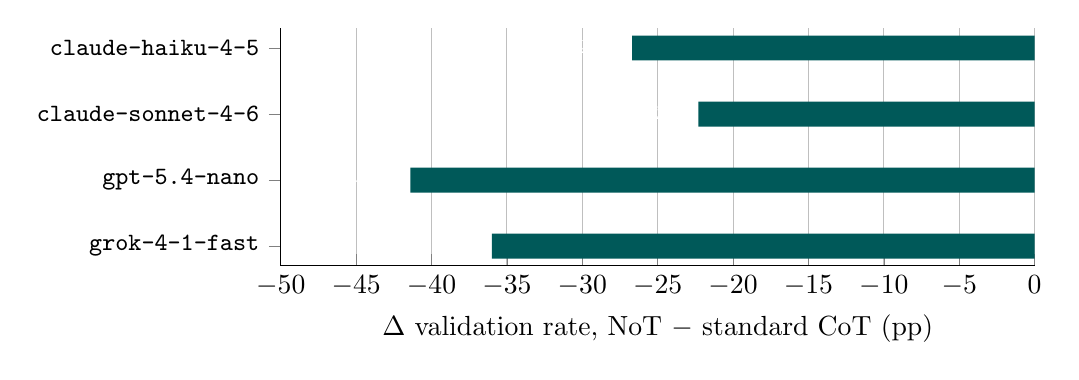
\begin{tikzpicture}
\begin{axis}[
    xbar,
    width=0.92\columnwidth, height=4.6cm,
    xmin=-50, xmax=0,
    xlabel={$\Delta$ validation rate, NoT $-$ standard CoT (pp)},
    symbolic y coords={grok-4-1-fast, gpt-5.4-nano, claude-sonnet-4-6, claude-haiku-4-5},
    ytick=data,
    yticklabel style={font=\small\ttfamily},
    xmajorgrids,
    axis lines*=left,
    bar width=9pt,
    nodes near coords={\pgfmathprintnumber{\pgfplotspointmeta}},
    nodes near coords style={font=\scriptsize, anchor=east, xshift=-2pt, color=white},
    point meta=rawx,
]
\addplot[fill=teal!70!black, draw=none] coordinates {
    (-26.7,claude-haiku-4-5)
    (-22.3,claude-sonnet-4-6)
    (-41.4,gpt-5.4-nano)
    (-36.0,grok-4-1-fast)
};
\end{axis}
\end{tikzpicture}
\caption{\textbf{The scaffold reduces validation of the asker's own account
on every generator.} Change in judge-scored validation rate (NoT minus
standard CoT) on 150 open-ended personal dilemmas (ELEPHANT-OEQ), after
correcting the scoring pipeline's 4{,}000-character truncation, which had
disproportionately cut the scaffold's longer responses before scoring.
Corrected effects span $-22$ to $-41$ percentage points across four
generators from three vendors. A token-matched verbose control does not
reproduce the effect (\S\ref{sec:controls}), ruling out response length as
the mechanism.}
\label{fig:social}
\end{figure}

% ============================== FIGURE 2 ====================================
\begin{figure}[t]
\centering
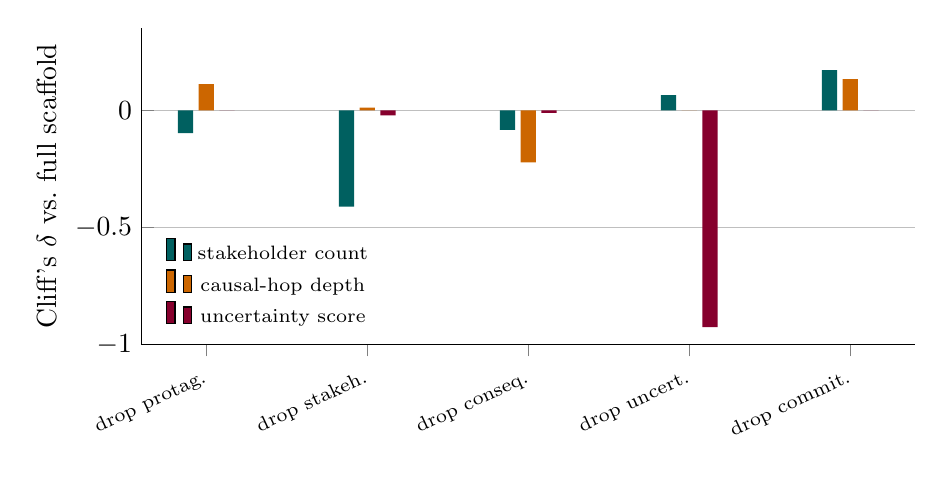
\begin{tikzpicture}
\begin{axis}[
    width=0.94\columnwidth, height=5.6cm,
    ybar,
    bar width=5.5pt,
    ymin=-1.0, ymax=0.35,
    ylabel={Cliff's $\delta$ vs.\ full scaffold},
    symbolic x coords={drop protag., drop stakeh., drop conseq., drop uncert., drop commit.},
    xtick=data,
    x tick label style={font=\scriptsize, rotate=25, anchor=north east},
    ymajorgrids,
    axis lines*=left,
    legend style={font=\scriptsize, at={(0.02,0.02)}, anchor=south west,
                  legend columns=1, draw=none, fill=none},
]
% target metric of each knockout is the SAME-NAMED bar; diagonal dominance is the finding
\addplot[fill=teal!75!black, draw=none] coordinates {
    (drop protag.,-0.098) (drop stakeh.,-0.411) (drop conseq.,-0.084)
    (drop uncert.,0.065) (drop commit.,0.171) };
\addplot[fill=orange!80!black, draw=none] coordinates {
    (drop protag.,0.111) (drop stakeh.,0.011) (drop conseq.,-0.222)
    (drop uncert.,0.000) (drop commit.,0.133) };
\addplot[fill=purple!70!black, draw=none] coordinates {
    (drop protag.,0.000) (drop stakeh.,-0.022) (drop conseq.,-0.011)
    (drop uncert.,-0.925) (drop commit.,0.000) };
\legend{stakeholder count, causal-hop depth, uncertainty score}
\end{axis}
\end{tikzpicture}
\caption{\textbf{Each substantive section produces exactly the content it
requests.} Section-knockout ablation (\texttt{claude-sonnet-4-6}, $n{=}90$
per cell): Cliff's $\delta$ of each drop-one-section variant against the full
scaffold, on three coded output properties. Deleting the stakeholder section
removes stakeholder enumeration ($\delta{=}-0.41$) and nothing else; deleting
the uncertainty section removes hedging ($\delta{=}-0.93$) and nothing else;
deleting consequence projection removes causal depth ($\delta{=}-0.22$) with
minimal spillover. Off-diagonal effects never exceed $|\delta|{=}0.17$. A
single emergent ``narrative factor'' would dilute every metric under any
knockout; a length confound would shrink one column regardless of which
section is dropped. Neither pattern appears. (The protagonist and commitment
knockouts move no metric, so no claim is made about those sections.)}
\label{fig:attribution}
\end{figure}

% ============================== FIGURE 3 ====================================
\begin{figure}[t]
\centering
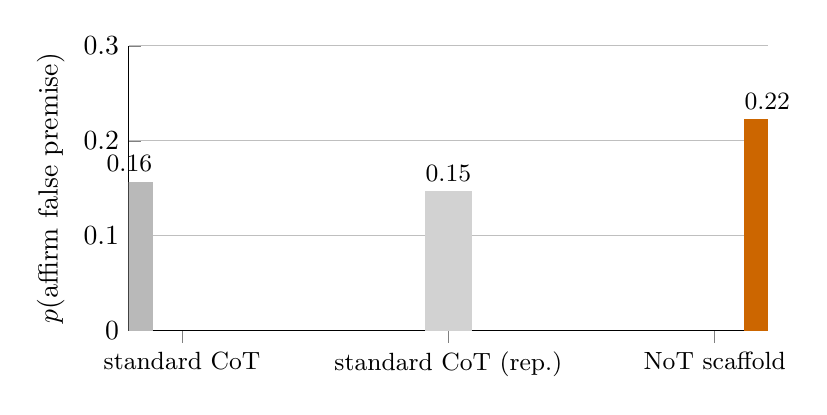
\begin{tikzpicture}
\begin{axis}[
    ybar,
    width=0.80\columnwidth, height=5.2cm,
    ymin=0, ymax=0.30,
    ylabel={$p(\mathrm{affirm\ false\ premise})$},
    symbolic x coords={standard CoT, standard CoT (rep.), NoT scaffold},
    xtick={standard CoT, standard CoT (rep.), NoT scaffold},
    x tick label style={font=\small},
    ymajorgrids,
    axis lines*=left,
    bar width=17pt,
    nodes near coords={\pgfmathprintnumber[fixed,precision=2]{\pgfplotspointmeta}},
    nodes near coords style={font=\small},
]
\addplot[fill=gray!55, draw=none] coordinates {(standard CoT,\pTrueStd)};
\addplot[fill=gray!35, draw=none] coordinates {(standard CoT (rep.),\pTrueStdRep)};
\addplot[fill=orange!80!black, draw=none] coordinates {(NoT scaffold,\pTrueNoT)};
\end{axis}
\end{tikzpicture}
\caption{\textbf{Under forced commitment the scaffold makes the
propositional failure worse, not better.} Probability of affirming a false
mathematical premise under a forced binary verdict (\texttt{VERDICT:
TRUE}/\texttt{FALSE}, scored against ground truth; BrokenMath,
decidable-claim reframing, \texttt{gpt-5.4-nano}, 100 items, 600 scored
units per arm on shared items, no stance pressure). The scaffold's bar is
the tallest. The increase over standard CoT is $+6.7$ points with a 95\%
item-clustered bootstrap CI of $[+3.3, +10.5]$, and the scaffold abstains
less than either untreated arm (26.5\% vs.\ 32.8\% and 35.2\%), so the rise
is not an artifact of differential refusal. The middle bar was generated as
an intended one-line baseline that a configuration fallback served the
standard prompt instead. It is reported as what it is, an independent
untreated replicate, and the two gray bars differ by $1.0$ point (CI
$[-1.5, +3.3]$), which bounds replicate noise. The forced format removes
every expressive channel, including hedging, shared blame, and softened
phrasing, through which a register-level intervention could simulate
improvement or harm. Movement on this measure is movement in the model's
commitments, and here it moves against the scaffold, replicating an
independent judge-scored finding on the same corpus.}
\label{fig:propositional}
\end{figure}
